\documentclass[12pt]{article}
\usepackage{graphicx}
\usepackage{amssymb}
\usepackage{epstopdf}
\usepackage{amsmath}
\usepackage{multicol}
\usepackage{tcolorbox}
\usepackage{geometry}
\usepackage{enumitem}
\usepackage{fancyhdr}

\DeclareGraphicsRule{.tif}{png}{.png}{`convert #1 `dirname #1`/`basename #1 .tif`.png}

\textwidth = 6.5 in
\textheight = 9 in
\oddsidemargin = 0.0 in
\evensidemargin = 0.0 in
\topmargin = -23pt
\headheight = 0.0 in
\headsep = 0.0 in
\parskip = 0.2in
\parindent = 0.0in
\pagestyle{fancy}
\pagenumbering{gobble}

\newtheorem{theorem}{Theorem}
\newtheorem{corollary}[theorem]{Corollary}
\newtheorem{definition}{Definition}
%\includegraphics [height=50mm, width=50mm]{PathInt.jpg}
\title{Title} 

\begin{document}
%INSTRUCTOR NOTES

 Name:
 \begin{center}\large{4.2 Optimization Part 1}\end{center}

\begin{enumerate}
\item Give an example of a function that does not have a global maximum or a global minimum value.

\vfill 

\item Find the global maximum and minimum for $\displaystyle f(x)=\frac{x+1}{x^2+3}$ on the interval $[-1,2]$.
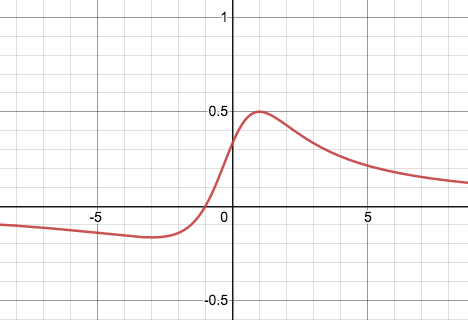
\includegraphics [scale=.45]{4_2_g1}

\item What value of $x$ minimizes $S$, where $S=5px+3qx^{2}-6pq$? (p and q are positive constants). Check your work using Desmos.
\vfill
\newpage

$\hspace{10px}$\\

\item What value of $t$ maximizes $y$, where $t>0$, and  $y=at^{2}e^{-bt}$?  ($a$ and $b$ are positive constants). Check your work using Desmos.
\vfill
\item (Taken from Hughes-Hallett, et. al.) When you cough, your windpipe contracts. The speed, $v$, at which the air comes out depends on the radius, $r$, of your windpipe. If $R$ is the normal (rest) radius of your windpipe, then for $0\leq r\leq R$, the speed is given by $v=a(R-r)r^2$, where $a$ is a positive constant. What value of $r$ maximizes the speed?
\vfill

\end{enumerate}
\end{document} 